Ante la necesidad de investigar las relaciones entre diferentes variables cuantitativas los análisis de regresión son una herramienta de frecuente uso en estadística, dado que simula un proceso o modelo que analiza este vínculo entre una variable dependiente y una o varias variables independientes. 

Una de las principales aplicaciones del análisis de regresión es la proyección con diferentes escenarios, teniendo en cuenta el grado de correlación sobre la variable dependiente y de esta manera construir una función que permita estimar el valor la variable de estudio. Ejemplos de implementación en python se pueden visualizar en el enlace \url{https://www.aprendemachinelearning.com/regresion-lineal-en-espanol-con-python/}.

\subsubsection{Forma analítica.}
La foma general analítica de una regresión no lineal tiene la forma matemática:
\begin{equation}
Y = f(X)+\epsilon
\end{equation}
donde:\\
\begin{tabular}{cp{14cm}}
$Y$ y $X$ & valores de salida y entrada multidimensionales.\\
$\epsilon$ & parámetro multidimensional correspondiente a los residuos.\\
$f$ & función de correlación.
\end{tabular}
Algunos problemas de regresión no lineal deben linealizarse mediante una transformación en la formulación del modelo, en el caso que nos ocupa en esta investigación esta será la manera de solucionar el hecho de que los datos correspondiente a la imagen son valores no negativos ($Y>0$) ya que son referidos a frecuencias resultado de la aplicación de métodos estadísticos sobre alguna propiedad de nuestro conjunto de datos. De lo cual tenemos:
\begin{equation}
\ln y = f(X)+\epsilon
\end{equation}
En el caso particular de esta investigación siempre la salida o imagen $y$ será referida a una variable simple y la forma de la función de entre $f$ será una polinomial, quedando entonces:
\begin{equation}\label{regresion}
\ln y = \sum_{i=0}^k (\alpha_{0i} + \alpha_{1i}\cdot x_i + \alpha_{2i}\cdot x_i^2 + \alpha_{3i}\cdot x_i^3 + \ldots+\alpha_{ni} \cdot x_i^n)+\epsilon
\end{equation}
el orden de la regresión está dado por $n$ y los valores $x_i$ serán las variables independientes de nuestro modelo, estos fueron integrados en una función en python implementando la paqueteria \texttt{sklearn} con la flexibilidad de cambiar los valores $k$ y $n$. %La función desarrollada para el uso en esta investigación se puede encontrar en el enlace \url{https://github.com/franky8939/DarkSUSY/blob/master/modules/machine_learning/regresion_lineal.py}.


\subsubsection{Redes neuronales.}
Las \textbf{RNA} son una estructura compuesta de un número de unidades interconectadas (neuronas artificiales), cada unidad posee una característica entrada/salida e implementa una computación local o función, la salida de cualquier unidad esta determinada, su interconexión con otras unidades, y posiblemente de sus unidades internas. La red desarrolla usualmente una funcionalidad por lo general a través de una o mas formas, por lo tanto es un arreglo masivo de elementos de procesamiento simple llamados neuronas, los cuales poseen un alto grado de interconectividad entre sus elementos, en los que la información puede fluir en cascada potenciando su capacidad para aproximar funciones, clasificar patrones y aumenta su inmunidad frente al ruido. 

La función desarrollada para el uso en esta investigación utiliza la paqueteria de \texttt{keras} y permite la flexibilidad de cambiar la cantidad de $k$ capas ocultas y los nodos $m_k$ que posee cada una de ellas.

%\url{https://github.com/franky8939/DarkSUSY/blob/master/modules/machine\_learning/regresion\_lineal\_ML.py}, 


\begin{figure}[h]
\centering
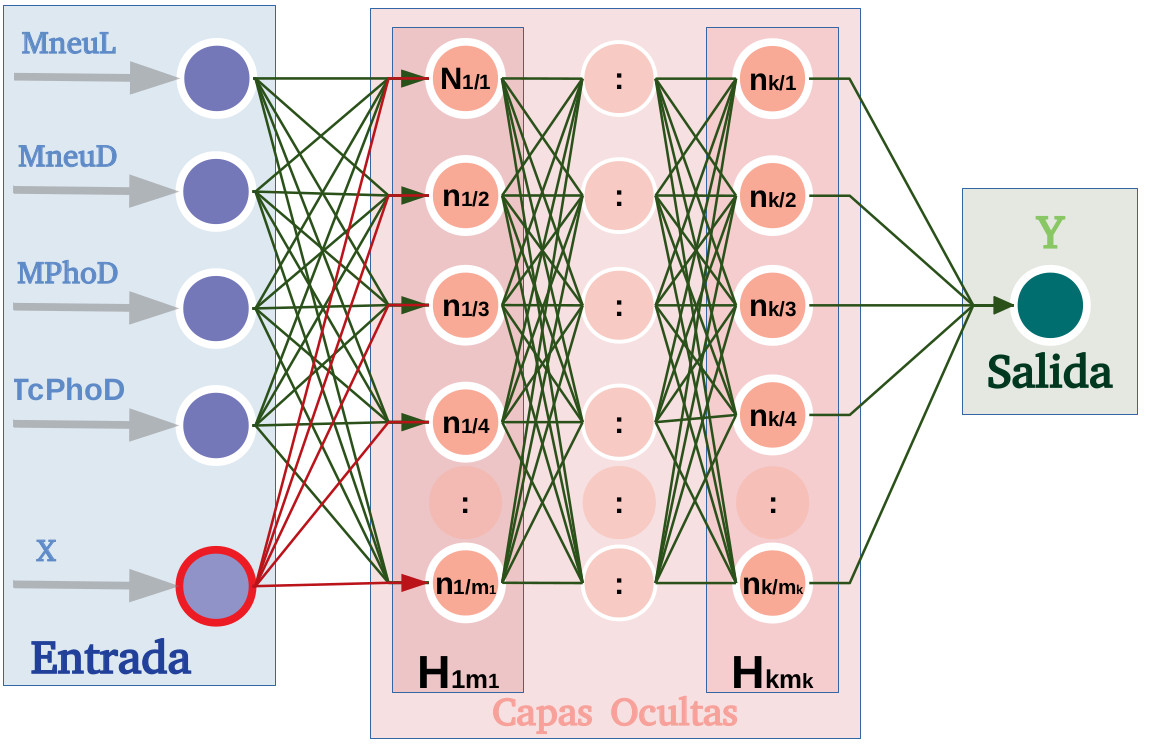
\includegraphics[width=.9\textwidth]{Simulacion/imagenes/neuronas.png}
\caption{Diagrama de la estructura general de la red neuronal.}
\label{neuronas}
\end{figure}

También se permite cambiar la dimensión de los datos de entrada para que estas coincidan con las necesidades futuras, siempre considerando como mínimas entradas las condiciones iniciales de generación y una variable extra en el caso de que sea necesario.

\subsubsection{Parámetros de confianza.}
Con el fin de determinar si el modelo es adecuado, se hace necesario utilizar conceptos de inferencia estadística tales como intervalos de confianza para los parámetros así como pruebas de bondad de ajuste. 

El parámetro \textbf{RMSE} (\textbf{R}oot \textbf{M}ean \textbf{S}quare \textbf{E}rror) es el error cuadrático medio o raíz de la desviación cuadrática media. Este mide la cantidad de error que hay entre dos conjuntos de datos, comparando un valor predicho y un valor observado o conocido, la ecuación que la describe es:
\begin{equation}
\mathbf{RMSE} ~ = ~ \sqrt{\dfrac{\sum_{i=1}^N |Y_{i}^{(sm)} -Y_{i}^{(real)}|^2}{N}} 
\end{equation}
donde $Y_{i}^{(sm)}$  es conjunto de datos predichos o simulados y $Y_{i}^{(real)}$ se corresponde con el conjunto de datos experimentales o observados.

La $\mathbf{RMSE}$ es siempre no negativa, y un valor de $0$ indicaría un ajuste perfecto a los datos. Dado que es una raíz cuadrada del promedio de errores cuadrados, este parámetro es proporcional al tamaño del error cuadrado; por lo tanto, los errores mayores tienen un efecto desproporcionadamente mas grande de aquí que sea sensible a los valores atípicos.

Otra prueba ampliamente utilizada es la prueba de correlación de Pearson o coeficiente de determinación ($\mathbf{R^2}$), esta se considera una prueba no paramétrica que mide la discrepancia entre una distribución observada y otra teórica, indicando en qué medida las diferencias existentes entre ambas, una de sus bondades es que es independiente de la escala de medida de las variables. La fórmula que da el estadístico es:
\begin{equation}
\mathbf{R^2} ~ = ~ \dfrac{\sum_{i=1}^N Y_{i}^{(sm)} Y_{i}^{(real)}}{\sqrt{(\sum_{i=0}^N Y_{i}^{(sm)})^2\cdot (\sum_{i=0}^N Y_{i}^{(real)})^2}}
\end{equation}  
El valor de este índice de correlación varía en el intervalo $[-1,~1]$, indicando el signo el sentido de la relación:
\begin{itemize_f}
\item[-] Si $\mathbf{R^2} = 1$, existe una correlación positiva perfecta. El índice indica una dependencia total entre las dos variables denominada relación directa: cuando una de ellas aumenta, la otra también lo hace en proporción constante.
\item[-] Si $0 < \mathbf{R^2} < 1$, existe una correlación positiva.
\item[-] Si $\mathbf{R^2} = 0$, no existe relación lineal. Pero esto no necesariamente implica que las variables son independientes: pueden existir todavía relaciones no lineales entre las dos variables.
\item[-] Si $-1 < \mathbf{R^2} < 0$, existe una correlación negativa.
\item[-] Si $\mathbf{R^2} = -1$, existe una correlación negativa perfecta. El índice indica una dependencia total entre las dos variables llamada relación inversa: cuando una de ellas aumenta, la otra disminuye en proporción constante.
\end{itemize_f}
%Además en estadística otro parámetro de gran importancia es el , este es un estadístico usado en el contexto de un modelo estadístico cuyo principal propósito es predecir futuros resultados o probar una hipótesis. El coeficiente determina la calidad del modelo para replicar los resultados, y la proporción de variación de los resultados que puede explicarse por el modelo.​

%Hay varias definiciones diferentes para R² que son algunas veces equivalentes. Las más comunes se refieren a la regresión lineal. En este caso, el R² es simplemente el cuadrado del coeficiente de correlación de Pearson, lo cual es sólo cierto para la regresión lineal simple. Si existen varios resultados para una única variable, es decir, para una X existe una Y, Z... el coeficiente de determinación resulta del cuadrado del coeficiente de determinación múltiple. En ambos casos el R² adquiere valores entre 0 y 1. Existen casos dentro de la definición computacional de R² donde este valor puede tomar valores negativos.2​ 
% \begin{tabular}{p{1.5cm}p{13cm}}

% \end{tabular}









